\section{Methode}
Für die Bestimmung der Evapotranspiration werden die Lysimeter- und Meteodaten mit MATLAB prozessiert. Da die Meteodaten in UTC und die Lysimeterdaten in MEZ vorliegen, müssen die Datensätze zuerst an eine Zeit angepasst werden. Zudem müssen die Einheiten so angepasst werden, dass sie auf die jeweiligen Berechnungsformeln passen.
\subsection {Lysimeter}

Ein Lysimeter ist eine Anlage, die zur Analyse von Wasser- und Stofftransport durch den Boden dient. Es besteht aus einem zylindrischen Topf, der mit Erde gefüllt ist. Am unteren Ende befindet sich ein Auslass für das versickerte Wasser und am Rand befinden sich auf verschiedenen Höhen diverse Messsonden. Wenn das Lysimeter auf einer Waage steht, kann zusätzlich die Gewichtsveränderung und somit der Wasserinput durch Niederschlag und der Wasserverlust durch die Evapotranspiration gemessen werden. Die Abbildung \ref{fig:lysimeter_ART}  zeigt die oberirdische Ansicht der Lysimter der ART. Eine Beschreibung der Komponenten der Lysimeter ist in der Abbildung \ref{fig:lysimeter_schema} zu sehen.\\

\begin{figure}[H]
\centering
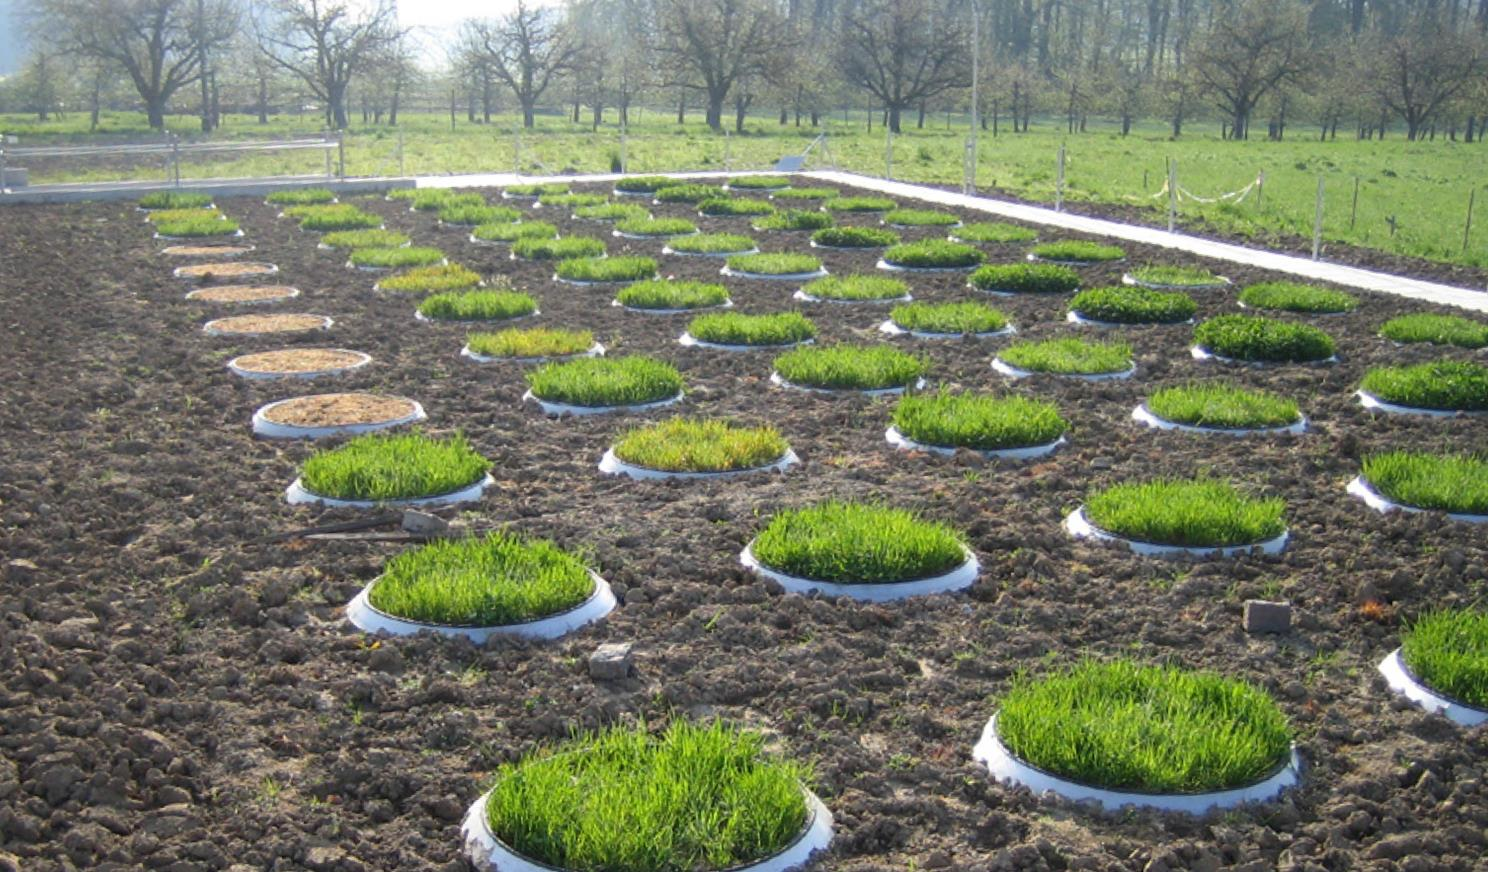
\includegraphics[width=0.8\textwidth]{figures/lysimeter_ART.jpg}
\caption{Lysimeteranlage der Forschungsanstalt Agroscope Reckenholz-Tänikon ART aus \cite{art}}
\label{fig:lysimeter_ART}
\end{figure}
 
\begin{figure}[H]
\centering
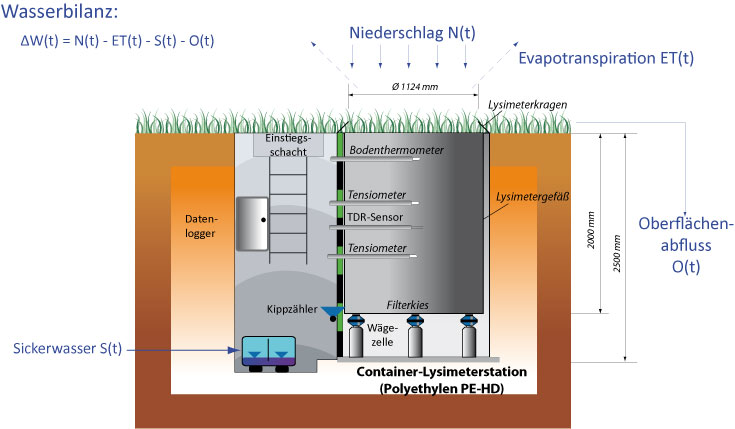
\includegraphics[width=0.8\textwidth]{figures/lysimeter_schema.jpg}
\caption{Schematische Darstellung eines Lysimeters aus \cite{ugt}}
\label{fig:lysimeter_schema}
\end{figure}


Zur Berechnung der Evapotranspiration mittels Lysimeterdaten wird die Bilanzformel (\ref{eq:wasserbilanz}) verwendet.


\begin{equation}
\label{eq:wasserbilanz}
AET=P-SW-\Delta W
\end{equation}
\begin{table}[H]
\centering
\begin{tabular}{ll}
AET& Reale Evapotranspiration [H/T]\\
P& Niederschlagsrate  [H/T]\\
SW & Sickerwasserrate  [H/T]\\
$\mathrm{\Delta W}$ & Änderung des Wasserspeichers  [H/T]\\
\end{tabular}
\end{table}


Die Änderung des Wasserspeichers wird aus der Gewichtsdifferenz des Lysimeters berechnet (\ref{eq:gewichtsänderung}).


\begin{equation}
\label{eq:gewichtsänderung}
\Delta W=\frac{\Delta m}{\rho_{Wasser}* A}
\end{equation}
\begin{table}[H]
\centering
\begin{tabular}{ll}
$\Delta W$ & Änderung der Wasserspeichers [H/T]\\
$\Delta m$ & Gewichtsänderung [kg]\\
$\mathrm{\rho_{Wasser}}$ & Dichte des Wassers $\mathrm{[kg/m^3]}$\\
A & Oberflläche des Lysimeters $\mathrm{[m^2]}$
\end{tabular}
\end{table}

Zur Bestimmung der Niederschlagsrate werden die Daten eines Niedeschlagsmessgeräts verwendet. Die Sickerwasserrate wird aus der Wassermenge, die unter dem Lysimeter aufgefangen wird, bestimmt.

\subsection{FAO Penman-Monteith-Methode}

Die Penman-Monteith-Methode kombiniert die beiden Ansätze der Massenbilanz und der Energiebilanz. Alle in der Formel enthaltenen Parameter können entweder direkt gemessen oder dann aus meteorologischen Daten berechnet werden. Die Methode impliziert, dass der aerodynamische und der Oberflächenwiderstand von der Oberflächenbepflanzung abhängig sind [vgl.\,Abb.\,\ref{fig:widerstand}]. 

\begin{figure}[H]
\centering
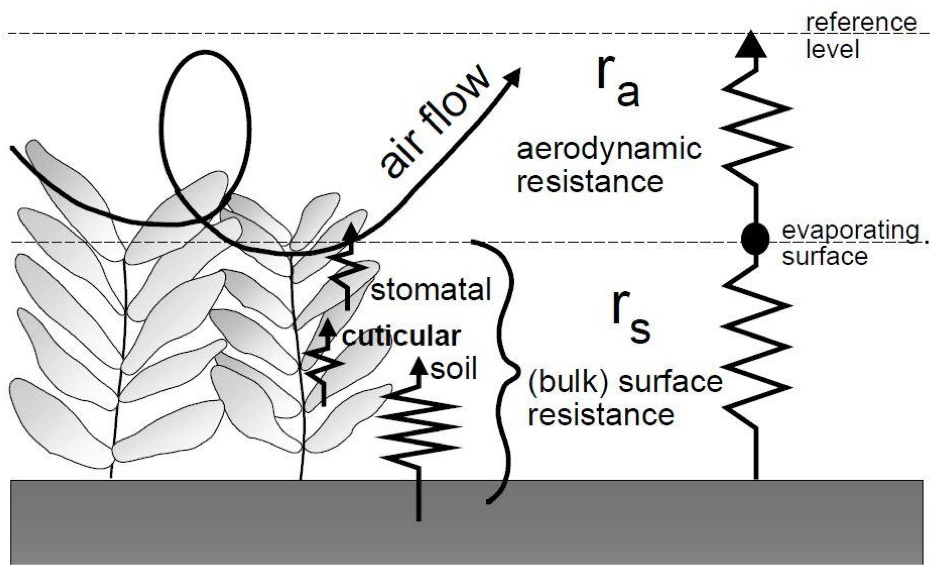
\includegraphics[width=0.8\textwidth]{figures/penman_widerstand.jpg}
\caption{Schematische Darstellung des aerodynamischen und des Oberflächenwiderstands in der Penman-Monteith-Methode (aus \cite{fao})}
\label{fig:widerstand}
\end{figure}

Der aerodynamische Widerstand beschreibt die Grösse, welche Wärme und Wasserdampf daran hindert , wegtransportiert zu werden. Diese hängt von der Windgeschwindigkeit und der Bodenrauigkeit ab. Der Oberflächenwiderstand beschreibt den Widerstand des Wasserdampfes, sich zwischen den transpirierenden Pflanzen und dem evaporierendem Boden zu bewegen. Dieser ist abhängig von Verhältnis der Blattfläche zur Bodenfläche und dem Stomatawiderstand eines gut bestrahlten Blattes. Unter Berücksichtigung dieser Einflüsse folgt die FAO\,Penman-Monteith-Formel für die Referenzfäche:

\begin{equation}
\label{eq:penman_ref}
ET_0=\frac{0.408\Delta \left(R_n-G\right)+\gamma \frac{900}{T+273}u_2\left(e_s-e_a\right)}{\Delta +\gamma\left(1+0.34u_2\right)}
\end{equation}
\begin{table}[H]
\centering
\begin{tabular}{ll}
$\mathrm{ET_0}$ & potentielle Referenzevapotranspiration $\mathrm{[mm/d]}$\\
$\mathrm{R_n}$ & Nettostrahlung $\mathrm{[MJ/m^2d]}$ \\
$\mathrm{G}$ & Bodenwärmefluss $\mathrm{[MJ/m^2d]}$\\
$\mathrm{\Delta}$ & Steigung der Sättigungsdampfdruckkurve $\mathrm{[kPa/^{\circ}C]}$\\
$\mathrm{\gamma}$ & Psychrometerkonstante $\mathrm{[kPa/^{\circ}C]}$\\
$\mathrm{T}$ & mittlere Temperatur in 2\,m Höhe $\mathrm{[^{\circ}C]}$\\
$\mathrm{u_2}$ & Windgeschwindigkeit in 2\,m Höhe $\mathrm{[m/s]}$\\
$\mathrm{e_s}$ & Sättigungsdampfdruck $\mathrm{[kPa]}$\\
$\mathrm{e_a}$ & aktueller Dampfdruck [kPa]\\
\end{tabular}
\end{table}

In den folgenden Berechnungen wird der Bodenwärmefluss allerdings vernachlässigt. Um die Evapotranspiration einer spezifischen Pflanze zu bestimmen, wird die Referenzevapotranspiration mit einem Pflanzenfaktor multipliziert. Es folgt daraus:

\begin{equation}
\label{eq:penman_spez}
ET_C=K_C*ET_0
\end{equation}
\begin{table}[H]
\centering
\begin{tabular}{ll}
$\mathrm{ET_0}$ & potentielle Referenzevapotranspiration $\mathrm{[mm/s]}$\\
$\mathrm{K_C}$ & Pflanzenfaktor [-]\\
$\mathrm{ET_C}$ & Evapotranspiration einer spezifischen Pflanze $\mathrm{[mm/s]}$\\\
\end{tabular}
\end{table}

Die Temperatur T kann aus den Meteodaten entnommen werden. Die übrigen Parameter müssen berechnet werden. Die FAO\,\cite{fao} gibt folgende Formeln:

\begin{description}
\item[Steigung der Sättigungsdampfdruckkurve]
\begin{equation}
\label{eq:delta}
\Delta=\frac{4098\left[0.6108*e^{\frac{17.27*T}{T+237.3}}\right]}{\left(T+237.3\right)^2}
\end{equation}
\begin{table}[H]
\centering
\begin{tabular}{ll}
$\mathrm{\Delta}$ & Steigung der Sättigungsdampfdruckkurve $\mathrm{[kPa/^{\circ}C]}$\\
T & mittlere Temperatur in 2\,m Höhe $\mathrm{[^{\circ}C]}$\\
\end{tabular}
\end{table}

\item[Nettostrahlung]

\begin{figure}[H]
\centering
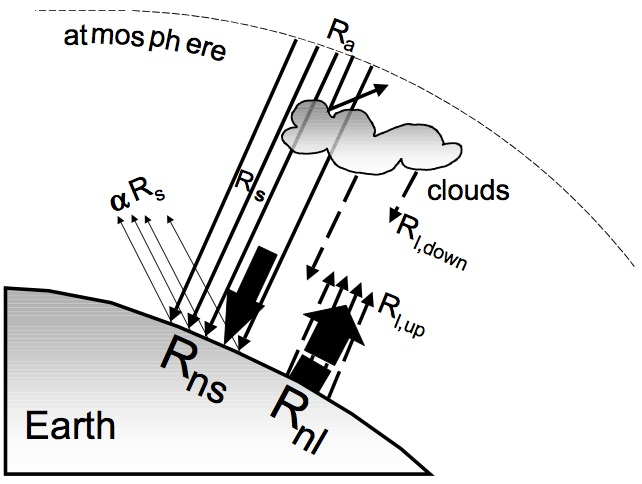
\includegraphics[width=0.8\textwidth]{figures/strahlung.jpg}
\caption{Schematische Darstellung der unterschiedlichen Strahlungsarten. $\mathrm{R_{s}}$ ist die kurzwellige Strahlung, $\mathrm{R_{l}}$ die langwellige Strahlung und $\mathrm{R_{a}}$ die atmosphärische Strahlung (aus \cite{fao})}
\label{fig:strahlung}
\end{figure}

\begin{equation}
\label{eq:rn}
R_n=0.77*R_s-\sigma\left[\frac{T_{max,K}^4+T_{min,K}^4}{2}\right]\left(0.34-0.14\sqrt{e_a}\right)\left(1.35\frac{R_s}{R_{s0}}-0.35\right)
\end{equation}
\begin{table}[H]
\centering
\begin{tabular}{ll}
$\mathrm{R_n}$ & Nettostrahlung $\mathrm{[MJ/m^2d]}$ \\
$\mathrm{R_s}$ & Kurzwellenstrahlung $\mathrm{[MJ/m^2d]}$ \\
$\mathrm{\sigma}$ & Stefan Boltzmann Konstante $\mathrm{[4.903*10^{-9}\,MJ/K^4m^2d]}$\\
$\mathrm{T_{max,K}}$ & maximale Temperatur während 24 h [K]\\
$\mathrm{T_{min,K}}$ & minimale Temperatur während 24 h [K]\\
$\mathrm{e_a}$ & aktueller Dampfdruck [kPa]\\
$\mathrm{R_{s0}}$ & Kurzwellenstrahlung ohne Wolkenbedeckung $\mathrm{[MJ/m^2d]}$\\
\end{tabular}
\end{table}

\begin{equation}
\label{eq:rs0}
R_{s0}=\left(0.75+2*10^{-5}z\right)*R_a
\end{equation}
\begin{table}[H]
\centering
\begin{tabular}{ll}
$\mathrm{R_s0}$ & Kurzwellenstrahlung ohne Wolkenbedeckung $\mathrm{[MJ/m^2d]}$\\
$\mathrm{R_a}$ & extraterrestrische Strahlung $\mathrm{[MJ/m^2d]}$ \\
z & Höhe über Meer [m]\\
\end{tabular}
\end{table}

\begin{equation}
\label{eq:Ra_short_period}
R_{a}=\frac{12 (60)}{\pi}G_{sc}*d_{r}[(\omega _{2}-\omega _{1})sin(\varphi)sin(\delta)+cos(\varphi)cos(\delta)(sin(\omega _{2})- sin(\omega _{1}))]
\end{equation}
\begin{table}[H]
\centering
\begin{tabular}{ll}
R$\mathrm{_{a}}$ & extraterrestrische Strahlung in einer Stunde (oder in kürzerem Zeitintervall) [MJ/m$\mathrm{^{2}}$h]\\
G$\mathrm{_{sc}}$ & Solarkonstante = 0.0820 MJ/m$\mathrm{^{2}}$min\\
d$\mathrm{_{r}}$ & inverse relative Distanz Sonne-Erde\\
$\mathrm{\delta}$ & solare Deklination [rad]\\
$\mathrm{\varphi}$ & geografische Breite [rad]\\
$\mathrm{\omega_{1}}$ & Sonneneinstrahlwinkel am Anfang der Zeitperiode [rad]\\
$\mathrm{\omega_{2}}$ & Sonneneinstrahlwinkel am Ende der Zeitperiode [rad]\\
\end{tabular}
\end{table}

\begin{equation}
\label{eq:Ra_long_period}
R_{a}=\frac{24 (60)}{\pi}G_{sc}*d_{r}[\omega _{s}sin(\varphi)sin(\delta)+cos(\varphi)cos(\delta)sin(\omega _{s})]
\end{equation}
\begin{table}[H]
\centering
\begin{tabular}{ll}
R$\mathrm{_{a}}$ & extraterrestrische Strahlung in einem Tag (oder in längerem Zeitintervall) [MJ/m$\mathrm{^{2}}$d]\\
G$\mathrm{_{sc}}$ & Solarkonstante = 0.0820 MJ/m$\mathrm{^{2}}$min\\
d$\mathrm{_{r}}$ & inverse relative Distanz Sonne-Erde [m]\\
$\mathrm{\delta}$ & solare Deklination [rad]\\
$\mathrm{\varphi}$ & geografische Breite [rad]\\
$\mathrm{\omega_{s}}$ & Sonneneinstrahlwinkel [rad]\\
\end{tabular}
\end{table}

\begin{equation}
\label{eq:dr}
d_r=1+0.033cos\left(\frac{2\pi}{365}J\right)
\end{equation}
\begin{equation}
\label{eq:delta_radiation}
\delta=0.409sin\left(\frac{2\pi}{365}J-1.30\right)
\end{equation}
\begin{table}[H]
\centering
\begin{tabular}{ll}
$\mathrm{d_r}$ & inverse Distanz Sonne-Erde [m]\\
$\mathrm{\delta}$ & solare Deklination [rad]\\
J & Korrekturfaktor (siehe \cite{fao} Annex 2 Table 2.5)\\
\end{tabular}
\end{table}

\begin{equation}
\label{eq:omega_s}
\omega_s=arccos[-tan(\varphi)tan(\delta)]
\end{equation}
\begin{table}[H]
\centering
\begin{tabular}{ll}
$\mathrm{\omega_s}$ & Sonneneinstrahlwinkel [rad]\\
$\mathrm{\varphi}$ & geografische Breite [rad]\\
$\mathrm{\delta}$ & solare Deklination [rad]\\
\end{tabular}
\end{table}

\begin{equation}
\label{eq:omega_i}
\omega_1=\omega-\frac{\pi t_i}{24}
\end{equation}
\begin{equation}
\omega_2=\omega+\frac{\pi t_i}{24}
\end{equation}
\begin{table}[H]
\centering
\begin{tabular}{ll}
$\mathrm{\omega}$ & Sonneneinstrahlwinkel [rad]\\
$\mathrm{t_i}$ & Zeitintervaldauer [h]\\
\end{tabular}
\end{table}

\begin{equation}
\label{eq:omega}
\omega=\frac{\pi}{12}[(t+0.06667(L_z-L_m)+S_c)-12]
\end{equation}
\begin{table}[H]
\centering
\begin{tabular}{ll}
$\mathrm{\omega}$ & Sonneneinstrahlwinkel [rad]\\
t & Zeit [h]\\
$\mathrm{L_z}$ & Längengrad in der Mitte der Zeitzone [rad]\\
$\mathrm{L_m}$ & Längengrad des Messpunktes [rad]\\
$\mathrm{S_c}$ & saisonaler Korrekturfaktor [h]\\
\end{tabular}
\end{table}

\begin{equation}
\label{eq:s_c}
S_c=0.1645sin(2b)-0.1255cos(b)-0.025sin(b)
\end{equation}
\begin{equation}
b=\frac{2\pi(J-81)}{364}
\end{equation}
\begin{table}[H]
\centering
\begin{tabular}{ll}
$\mathrm{S_c}$ & saisonaler Korrekturfaktor [h]\\
J & Korrekturfaktor (siehe \cite{fao} Annex 2 Table 2.5)\\
\end{tabular}
\end{table}

\item[Psychrometerkonstante]
\begin{equation}
\label{eq:gamma}
\gamma=0.665*10^{-3} P
\end{equation}
\begin{table}[H]
\centering
\begin{tabular}{ll}
$\mathrm{\gamma}$ & Psychrometerkonstante $\mathrm{[kPa/^{\circ}C]}$\\
P & Atmosphärendruck [kPa]\\
\end{tabular}
\end{table}

\item[Windgeschwindigkeit in 2 m Höhe]
\begin{equation}
\label{eq:u2}
u_2=u_z\frac{4.87}{ln(67.8z-5.42)}
\end{equation}
\begin{table}[H]
\centering
\begin{tabular}{ll}
$\mathrm{u_2}$ & Windgeschwindigkeit in 2\,m Höhe $\mathrm{[m/s]}$\\
$\mathrm{u_z}$ & Windgeschwindigkeit in z\,m Höhe $\mathrm{[m/s]}$\\
z & Messhöhe [m]\\
\end{tabular}
\end{table}

\item[aktueller Dampfdruck]
\begin{equation}
\label{eq:ea}
e_a=0.6108*e^{\frac{17.27T}{T+273.3}}
\end{equation}
\begin{table}[H]
\centering
\begin{tabular}{ll}
$\mathrm{e_a}$ & aktueller Dampfdruck $\mathrm{[kPa]}$\\
T & mittlere Temperatur in 2\,m Höhe $\mathrm{[^{\circ}C]}$\\\end{tabular}
\end{table}

\item[Sättigungsdampfdruck]
\begin{equation}
\label{eq:es}
e_s=\frac{e_a(T_{max})+e_a(T_{min})}{2}
\end{equation}
\begin{table}[H]
\centering
\begin{tabular}{ll}
$\mathrm{e_s}$ & Sättigungsdampfdruck $\mathrm{[kPa]}$\\
T & mittlere Temperatur in 2\,m Höhe $\mathrm{[^{\circ}C]}$\\
\end{tabular}
\end{table}


\end{description}

\subsection{Turc-Methode}
Das Modell von Turc ist für Frankreich und Nordafrika entwickelt worden und ist nur für Temperaturen über 0\,$\mathrm{^{\circ}C}$ definiert.

Es ist ein strahlungsbasiertes empirisches Modell. Als Input Parameter wird aber nicht nur die globale Strahlung, sondern auch die Temperatur benötigt. Das Modell ist nur für Temperaturen im positiven Bereich anwendbar und wird ungenau bei tiefen Temperaturen. Die potentielle Evapotranspirationsrate berechnet sich zu:

\begin{equation}
\label{eq:turc}
PET=0.31C\left(R_G+2.094\right)*\frac{T}{T+15}
\end{equation}
\begin{table}[H]
\centering
\begin{tabular}{ll}
PET & Evapotranspirationsrate nach Turc  $\mathrm{[mm/d]}$\\
T & mittlere Lufttemperatur im gegebenen Zeitinterval $\mathrm{[^{\circ}C]}$\\
$\mathrm{R_G}$ & globale Strahlung $\mathrm{[MJ/m^2\,d]}$\\
C & für rel. Luftfeuchtigkeit RH $\geq$ 50\% = 1\\
\end{tabular}
\end{table}
Für eine rel. Luftfeuchtigkeit < 50\% gilt:
\begin{equation}
\label{eq:turc_c}
C=1+\left(\frac{50-RH}{70}\right)
\end{equation}
\begin{table}[H]
\centering
\begin{tabular}{ll}
RH& durchschnittliche rel. Luftfeuchtigkeit [\%]\\
\end{tabular}
\end{table}

\subsection{Ivanov-Methode}
Das Modell von Ivanov ist eine modifizierte Version des Modells von Turc. Es kann für die Abschätzung der Evapotranspirationsrate bei tieferen Temperaturen in den Monaten November bis Februar genutzt werden und ist ein temperaturbasiertes Modell. Für die Berechnung der täglichen Evapotranspiration wird folgende Formel benutzt:

\begin{equation}
\label{eq:ivanov_d}
PET=0.000036(25+T)^2(100-RH)
\end{equation}
\begin{table}[H]
\centering
\begin{tabular}{ll}
PET & Evapotranspirationsrate nach Ivanov  $\mathrm{[mm/d]}$\\
T & mittlere Lufttemperatur im gegebenen Zeitinterval $\mathrm{{^\circ}C]}$\\
RH& durchschnittliche rel. Luftfeuchtigkeit [\%]\\
\end{tabular}
\end{table}

Für die monatliche Evapotranspiration wird folgende Formel verwendet:

\begin{equation}
\label{eq:ivanov_m}
PET=0.0011(25+T)^2(100-RH)
\end{equation}
\begin{table}[H]
\centering
\begin{tabular}{ll}
PET & Evapotranspirationsrate nach Ivanov  $\mathrm{[mm/Mt]}$\\
T & mittlere Lufttemperatur im gegebenen Zeitinterval $\mathrm{{^\circ}C]}$\\
RH& durchschnittliche rel. Luftfeuchtigkeit [\%]\\
\end{tabular}
\end{table}

\subsection{Sensitivitätsanalyse}

Die Sensitivitätsanalyse wird für die Penman-Monteith Formel\,(\ref{eq:penman_ref}), die Methode nach Turc\,(\ref{eq:turc}) und die Methode nach Ivanov\,(\ref{eq:ivanov_d}) durchgeführt. Dazu wird jeweils ein Parameter um $\pm$10\% verändert und die Auswirkungen auf die berechnete Evapotranspiration berechnet. Für die gemessen Grössen wurden Werte festgesetzt und daraus die weiteren Parameter berechnet. Für den Sättigungsdampfdruck, wird eine minimale Temperatur von $\mathrm{10\,^{\circ}C}$ und eine maximale Temperatur von $\mathrm{20\,^{\circ}C}$ angenomen.




